% Nama Kelompok : Linux
% Kelas : D4 TI 1A
% 1. Kadek Diva Krishna Murti (1174006)
% 2. Duvan Silalahi (1174011)
% 3. Oniwaldus (1174005)
% 4. Choirul Anam (1174004)
% 5. Sri Rahayu (1174015)
% 6. Ilham Habibi (1174028)


\begin{figure}[ht]
\centerline{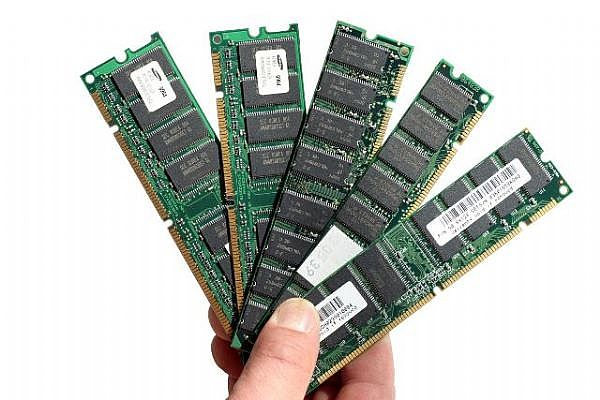
\includegraphics[width=1\textwidth]{figures/memori.jpg}}
\caption{Contoh gambar memori.}
\label{memori}
\end{figure}

Memori disebut juga sebagai memori fisik merupakan suatu istilah generik yang merujuk pada media penyimpanan data sementara pada komputer. Setiap program dan data yang sedang diproses oleh prosesor akan disimpan di dalam memori fisik. Data yang disimpan pada memori fisik bersifat sementara, karena data yang disimpan di dalamnya akan tersimpan selama komputer tersebut masih dialiri daya dengan kata lain, komputer itu masih dalam keadaan hidup. Ketika sebuah komputer dimatikan atau direset, data yang disimpan dalam memori fisik akan hilang. Oleh sebab itulah sebelum anda mematikan komputer Anda, anda harus benar - benar menyimpan semua data yang belum anda simpan ke media penyimpanan permanen umumnya berbasis disk, seperti hard disk atau floppy disk, sehingga pada saat komputer anda dihidupkan kembali data tersebut dapat dibuka kembali di lain kesempatan. Memori fisik biasanya diterapkan dalam bentuk Random Access Memory (RAM), yang bersifat dinamis (DRAM). Disebut Random Access adalah karena akses terhadap tempat-tempat di dalamnya dapat dilakukan secara acak atau random, bukan secara berurutan atau sekuensial. Meskipun demikian, kata random access dalam RAM ini sering terjadi salah paham. Sebagai contoh, memori yang hanya dapat dibaca seperti Read Only Memory (ROM) juga bisa diakses secara random, tetapi ia dibedakan dengan RAM karena ROM dapat menyimpan data tanpa kebutuhan daya dan tidak dapat ditulisi sewaktu-waktu. Tidak hanya itu, hard disk sebagai media penyimpanan juga bisa diakses secara random, namun hardisk tidak dikategorikan kedalam sebuah khusuRandom Access. Ini adalah contoh gambar memori \ref{memori}

\section{Sejarah Memori}
Perkembangan micro computer atau yang biasanya sering disebut juga dengan nama PC (Personal Computer) yang sedemikian pesat tentunya tidak lepas dari kebutuhan manusia akan informasi yang harus diolah oleh PC. Perkembangan teknologi tersebut termasuk dalam teknologi perangkat keras, perangkat lunak, serta fungsi atau algoritma yang digunakan dalam memproses informasi yang diolah tersebut.
Pada awal ditemukannya PC banyak orang menganggap PC sebagai barang yang mahal atau mewah, namun kini anggapan itu tidak berlaku lagi karena hampir semua orang sudah memilikinya. Bisa dikatakan, orang yang tidak mengenal komputer pada zaman sekarang akan dicap sebagai orang yang gagap teknologi. Jika pada saat itu PC yang diotaki oleh prosessor Intel 8088 hanya mampu berjalan dengan kemampuan kecepatan 4,77 MHz yang digunakan untuk menajalankan program pengolah kata dalam pembuatan dan mengubah dokumen, spreadsheet sederhana untuk mengerjakan pekerjaan akuntansi maupun bisnis, dan program database sederhana serta sedikit program pendidikan dan game yang juga masih sangat sederhana. Pada masa sekarang PC yang diotaki Intel Pentium 4 mampu berjalan dengan kecepatan 2GHz, bahkan baru - baru ini Intel Corp melalui ajang Intel Developer Forum-nya, telah menunjukkan demo prosessor Intel berkecepatan 3,5GHz Suatu penemuan teknologi yang cukup fantastis dan muktakhir. Namun pada perkembangan selanjutnya kemampuan PC tidak selalu ditentukan oleh perkembangan prosessor semata, bisa juga faktor lainnya, seperti teknologi chipset, memori, kartu VGA, perangkat media simpan, dan sebagainya. Semua perangkat saling berevolusi dan berkembang ke arah yang lebih baik untuk bersama - sama membangun suatu sistem PC yang tangguh. Perkembangan kemampuan prosessor yang begitu pesat tentunya harus diimbangi dengan peningkatan kemampuan memori. Memori dibutuhkan oleh prosessor sebagai tempat penyimpan data atau informasi sekaligus sebagai penyimpan hasil dari perhitungan yang dilakukan oleh prosessor itu sendiri, sehingga kemampuan memori dalam mengelola data tersebut sangatlah penting. Percuma saja apabila kita memliki sebuah sistem PC dengan prosessor berkecepatan tinggi apabila tidak diimbangi dengan kemampuan memori yang sepadan. Ketidaktepatan dalam perpaduan kemampuan prosessor dengan memori dapat menyebabkan inefisiensi bagi keduanya. Andaikan apabila kita mempunyai sebuah prosessor yang mampu mengelola arus data sebanyak 100 instruksi per detiknya, sementara kita memiliki memori dengan kemampuan menyalurkan data ke prosessor sebesar 50 instruksi per detiknya. Yang terjadi adalah sistem akan mengalami ketidakseimbangan yang disebabkan perbedaan kecepatan kerja antara prosessor dengan memori yang berarti prosessor harus menunggu data dari memori dan menyebabkan data yang seharusnya dapat dikerjakan dalam waktu 1 detik, menjadi 2 detik karena kemampuan memori yang terbatas. 

\section{Penggunaan memori}
Komponen utama dalam suatu sistem komputer adalah Arithmetic and Logic Unit (ALU), Control Circuitry, Storage Space dan piranti Input atau Output. Tanpa adanya sebuah memori, sebuah komputer hanya akan berfungsi sebagai perangkat pemroses sinyal digital saja, contohnya kalkulator atau media player. Yang membuat sebuah komputer dapat disebut sebagai komputer multi-fungsi (general-purpose)  adalah kemampuan  dari memori untuk menyimpan data, instruksi serta informasi. Komputer merupakan sebuah piranti digital oleh karena itu, informasi yang disajikan oleh komputer yaitu menggunakan sistem bilangan biner atau binary. File yang berupa teks, angka, gambar, suara dan video akan dikonversikan menjadi sekumpulan bilangan biner atau binary digit atau disingkat bit. Sekumpulan bilangan - bilangan biner dikenal dengan istilah BYTE, dimana  1 bita sama dengan 8 bit, 1 bit sama dengan 1 karakter, 1 kilobita sama dengan 1024 bita, dan bps sama dengan bit per second, 1 kbps sama dengan 1000 bps, 1 mbps sama dengan 1.000.000 bps. Semakin besar suatu ukuran memori maka semakin banyak pula informasi yang dapat disimpan di dalam media penyimpanan komputer.

\section{Jenis - Jenis Memori}

\subsection{Jenis Memori Yang Populer}

Berikut ini beberapa jenis memori yang banyak digunakan pada saat ini sebagai berikut:

\begin{enumerate}

\item RAM (Random Acces Memory) adalah memory sebagai tempat penyimpanan sementara pada saat komputer di jalankan dan dapat di akses secara acak atau random. Fungsi dari RAM adalah mempercepat pemrosesan data pada komputer. Semakin tinggi jumlah RAM yang Anda miliki, semakin cepat pula kemampuan komputer Anda dalam mengeksekusi.
Jenis Memory RAM :

\begin{itemize}

\item EDORAM (Extended Data Out RAM)  
\item SDRAM (Synchronous Dynamic RAM)  
\item DDR SDRAM (Double Data Rate Synchronous Dynamic RAM) 
\item RDRAM (Rambus Dynamic RAM)

\end{itemize}	

\item Menurut artikel yang berjudul Evolusi Komputer, Kinerja Komputer Dan Interconnection Networks Dalam Perkembangan Dunia Teknologi Informatika menyebutkan bahwa Registers adalah media penyimpan internal CPU yang digunakan saat proses pengolahan data. Memori ini bersifat sementara, biasanya hanya digunakan untuk menyimpan data saat diolah ataupun data untuk pengolahan selanjutnya. Sistem dan bus yang menghubungkan komponen-komponen eksternal CPU dengan sistem lain, seperti memori utama serta piranti masukan atau keluaran dan juga menghubungkan komponen – komponen internal CPU dengan system lain, seperti Arimathics Logics Unit, Unit Control, dan Registers system koneksi dan bus tersebut disebut CPU Interconnections. \cite{junior2016evolusi}

\item Menurut artikel yang berjudul Evolusi Komputer, Kinerja Komputer Dan Interconnection Networks Dalam Perkembangan Dunia Teknologi Informatika menyebutkan bahwa Read Only Memory disingkat ROM merupakan memori yang tidak dapat dihapus isinya, hanya dapat dibaca, dan sudah diisi oleh pabrik pembuat komputer atau bisa dikatakan tidak bisa diprogram kembali. Sebagian perintah pada ROM akan dipindahkan ke RAM. Perintah yang ada di ROM antara lain, perintah untuk menampilkan pesan dilayar, perintah untuk membaca Sistem Operasi dari disk, dan perintah untuk mengecek semua peralatan yang ada di Unit Sistem.
Perkembangan ROM (Read Only Memory)
- Programble ROM disingkat PROM merupakan ROM yang bisa diprogram kembali dengan catatan hanya bisa diprogram 1 x.
- Re-Programble ROM disingkat RPROM merupakan ROM yang bisa diprogram ulang sesuai dengan yang kita inginkan.
- Eraseble Programble ROM disingkat EPROM merupakan ROM yang dapat dihapus dan diprogram kembali tetapi cara penghapusannya dengan menggunakan Sinar Ultraviolet.
- Electrically Eraseble Programble ROM disingkat EEPROM merupakan ROM yang bisa diprogram dengan Teknik Elektronik. \cite{junior2016evolusi}

\item Dynamic RAM disingkat DRAM merupakan salah satu jenis RAM yang harus disegarkan secara berkala oleh CPU supaya data yang terkandung di dalamnya tidak hilang. DRAM merupakan salah satu tipe RAM yang terdapat dalam PC.
Compmentary Meta-Oxyde Semiconductor disingkat CMOS merupakan jenis chip yang memerlukan daya listrik dari baterai. Chip ini berisi memori 64-byte yang isinya dapat diganti. Chip ini biasanya mengatur berbagai pengaturan - pengaturan dasar yang terdapat 
pada perangkat komputer, seperti piranti yang digunakan untuk memuat sistem operasi dan termasuk pula tanggal dan jam sistem. CMOS merupakan bagian dari ROM.

\item Sychronous Dynamic RAM disingkat SDRAM merupakan kelanjutan dari DRAM tetapi memiliki kecepatan yang lebih tinggi daripada DRAM dan telah disinkronisasi oleh clock sistem. DRAM ini cocok digunakan untuk sistem dengan bus yang memiliki kecepatan sampai 100 MHz.

\item Dual In-line Memory Module disingkatan DIMM dari  berkapasitas 168 pin, kedua belah modul memori ini aktif, setiap permukaan adalah 84 pin. Berbeda dengan SIMM yang berfungsi hanya pada sebelah modul saja. Mensuport 64 bit penghantaran data. SDRAM
(Synchronous DRAM) menggunakan DIMM dan merupakan penganti dari DRAM, FPM (fast Page Memory) dan EDO. SDRAM memiliki fungsi untuk mengatur (synchronizes) memori supaya setara dengan CPU clock supaya pemindahan data yang dilakukan dapat dilakukan secara cepat. Terdapat dalam dua kecepatan yaitu 100MHz (PC100) dan 133MHz (PC133). DIMM 168 PIN. DIMM merupakan jenis RAM yang populer dan paling banyak terdapat di pasaran.

\item Cache merupakan memori yang berkapasitas terbatas, namun memori ini memiliki kecepatan  yang tinggi dan lebih mahal dibandingkan memory utama. Cache ini terletak di antara register pemroses dan memori utama, dan memiliki fungsi agar pemroses tidak langsung mengacu kepada memori utama tetapi langsung di cache memory yang kecepatan aksesnya lebih tinggi, metode ini akan meningkatkan kinerja sistem. Cache memori merupakan salah satu tipe RAM tercepat yang pernah ada, dan digunakan oleh CPU, hard drive, dan beberapa pernah lainnya.

\item Magnetik Disk merupakan sebuah piringan bundar yang terbuat dari bahan tertentu seperti, logam atau plastik dengan permukaan dilapisi bahan - bahan yang dapat di magnetisasi. Mekanisme baca atau tulis menggunakan head atau kepala baca atau tulis yang dimana merupakan sebuah kumparan pengkonduksi (conducting coil ). Tampilan luar head bersifat stasioner sedangkan piringan disk berputar sesuai kontrolnya. Disk memiliki dua metode layout data, yaitu  constant angular velocity dan multiple zoned recording. Disk diorganisasikan dalam bentuk berupa cincin – cincin
Konsentris yang disebut track. Tiap track pada disk dipisahkan oleh gap. Gap digunakan sebagai pencegah atau mengantisipasi kesalahan penulisan maupun pembacaan yang disebabkan melesetnya head atau karena interferensi medan magnet. Sejumlah bit yang sama akan menempati track - track yang tersedia. Semakin dalam maka kerapatan dari disk akan bertambah besar. Biasanya data yang dikirim ke memori dalam bentuk blok - blok dan umumnya blok - blok tersebut lebih kecil kapasitasnya dari pada track. Blok - blok data yang disimpan dalam disk yang berukuran blok, yang disebut sektor. Sehingga track biasanya terisi beberapa sektor, umumnya 10 hingga 100 sektor tiap tracknya. Cara mekanisme pembacaan maupun penulisan pada disk dengan Head harus bisa mengidentifikasi titik awal atau posisi - posisi sektor maupun track. Caranya data yang disimpan akan diberi header data tambahan yang menginformasikan letak sektor dan track suatu data. Tipe memori Teknologi Ukuran Waktu akses Cache Memory semikonduktor RAM 128-512 KB 10 ns. Memori Utama semikonduktor RAM 4-128 MB 50 ns. Disk magnetik Hard Disk Gigabyte 10 ms, 10MB/det. Disk Optik CD-ROM Gigabyte 300ms, 600KB/det Pita magnetik Tape 100 MB De.

\end{enumerate}

\subsection {Jenis Memori Berdasarkan Memori}


Menurut artikel yang berjudul Pengantar Komputer dan Perkembangannya menyebutkan bahwa berikut ini adalah dua jenis memori berdasarkan fungsinya, yaitu :

\begin{enumerate}

\item Primary Memory, memori ini dipergunakan untuk menyimpan instruksi dan data dari program - program yang sedang dijalankan. Primary memory biasanya juga 
disebut sebagai RAM. Ciri - ciri dari memori primer itu sendiri adalah sebagai berikut :  

\begin{itemize}


\item Volatil (informasi ada selama komputer sedang bekerja. Ketika sebuah komputer dimatikan, informasi yang disimpan juga menghilang)  
\item Kecepatan tinggi  
\item Akses random (acak)  
\item I/O Device memori

\end{itemize}

\item Secondary Memory, dipergunakan untuk semikonduktor RAM 4-128 MB 50 ns. Disk magnetik Hard Disk Gigabyte 10 ms, 10MB/det. Disk Optik CD-ROM Gigabyte 300ms, 600KB/det Pita magnetik Tape 100 MB De. menyimpan data atau program biner secara permanen. Ciri - ciri dari memori sekunder adalah sebagai berikut:  

\begin{itemize}

\item Non volatil atau persisten  
\item Kecepatan relatif rendah (dibandingkan memori primer)  
\item Akses random atau sekuensial  

\end{itemize}

Contoh memori sekunder : floppy, harddisk, CD ROM, magnetic tape, optical disk, dan lain - lain. Dari seluruh contoh yang disebutkan diatas, yang memiliki mekanisme akses sekuensial adalah magnetic tape. \cite{dwi2010pengantar}

\end{enumerate}

\section {Pembagian memori}
Pada arsitektur komputer yang dibuat oleh arsitektur Von Neumann seperti, kecepatan dan kapasitas memori dapat dibagi dengan menggunakan hierarki memori. Hierarki memori ini diurutkan dari harga tiap bit memori-nya mulai dari yang paling tinggi atau mahal hingga yang paling rendah atau murah, disusun dari yang paling kecil kapasitasnya hingga paling besar kapasitasnya, dan dibuat dari jenis - jenis memori yang paling cepat hingga yang paling lambat.
